%&latex
%
\documentclass[../template.tex]{subfiles}
\begin{document}

\lesson{8}{3/4/20}

\section{Basic Limit Theorem of Markov Chains}
We are finally able to formalize and \textit{prove} the intuitive fact that the \textit{long-run} probability of returning to a state $i$ is the \textit{reciprocal} of the average return time of $m_i$: that is, if the system is at $i$ every $m_i$ steps, then it spends $1/m_i$ of the total time in $i$, and so if we inspect the state at a random step (of a \textit{infinitely long} experiment) we will find the system at $i$ with probability $1/m_i$. Moreover, we will also find the appropriate conditions that are necessary for this result to hold.  

\medskip

Consider a \textbf{recurrent} state $i$. As we have seen before, the first return time $R_i$ can be defined as:
\begin{align*}
    R_i = \min\{n \geq i; X_n = i\}
\end{align*}
and is distributed according to:
\begin{align*}
    f_{ii}^{(n)} = \mathbb{P}\{R_i = n | X_0 = i\} = \mathbb{P}\{X_n = i, X_\nu \neq i \> \forall \nu = 1,\dots,n|X_0 = i\} 
\end{align*} 
Since the state $i$ is recurrent, $f_{ii} = \sum_{n=1}^\infty f_{ii}^{(n)} = 1$, and so $R_i$ is a finite-valued random variable. In other words, $R_i$ can never be infinite, since the system will return to $i$ \textit{for sure}. More precisely, the probability of $R_i$ being arbitrarily high \textit{vanishes}. 

\medskip

The mean duration between visits to state $i$ is the expectation of $R_i$:
\begin{align*}
    m_i = \mathbb{E}[R_i | X_0 = i] = \sum_{n=1}^\infty n f_{ii}^{(n)}
\end{align*}
In other words, the system \textit{on average} returns to $i$ once every $m_i$ units of time.  

\medskip

Note that the fact that $R_i$ is a finite-valued random variable does \textbf{not} prevent $m_i$ from being infinite. This in fact happens if $\mathbb{P}[R_i = n]$ decreases \textit{sufficiently slowly} as $n \to \infty$.   

\begin{thm} \textbf{Basic limit theorem of Markov Chains}\label{thm:basic-limit}

    \begin{enumerate}[label=(\alph*)]
        \item Consider a \textbf{recurrent}, \textbf{irreducible}, \textbf{aperiodic} Markov chain. Let $P_{ii}^{(n)}$ be the probability of entering state $i$  at the $n$-th transition, with $n \in \mathbb{N}$, given that the initial state is $i$ ($X_0 = i$). Let $f_{ii}^{(n)}$ be the probability of first returning to state $i$ at the $n$-th transition. Then:
        \begin{align*}
            \lim_{n \to \infty} P_{ii}^{(n)} = \frac{1}{\sum_{n=1}^\infty n f_{ii}^{(n)}} = \frac{1}{m_i}  
        \end{align*}  
        \item Also:
        \begin{align*}
            \lim_{n \to \infty} P_{ji}^{(n)} = \pi_i =\lim_{n \to \infty} P_{ii}^{(n)} = \frac{1}{m_i} 
        \end{align*}
        for all states $j$.
    \end{enumerate}
\end{thm}

The proof is referred to a later chapter.

\medskip

Note that theorem \ref{thm:basic-limit} can be applied also to \textbf{aperiodic} \textbf{recurrent classes} in a Markov Chain. In fact, we noted that different classes can only be linked by \textit{one-way} transitions - meaning that after leaving a class $C$, the system cannot return in it. So a \textit{recurrent class} must necessarily be isolate, i.e. such that $P_{ij}^{(n)} = 0$ for all $i \in C$, $j \notin C$, and for all $n$. So we can consider the submatrix $\norm{\textbf{P}_{ij}}$, with $i,j \in C$, as the transition probability matrix of a separate \textbf{irreducible} Markov Chain, for which the basic limit theorem directly applies. 

\medskip

Depending on the finiteness of $m_i$, we distinguish two cases:
\begin{itemize}
    \item If the average return time $m_i$ is \textbf{finite}, then $\lim_{n \to \infty} P_{i i}^{(n)} > 0$, and the same applies to all states $j \leftrightarrow i$. This means that $\pi_j > 0$ for every $j$, and so all states in the \textit{aperiodic recurrent class} continue to be visited in the long run. Classes with this property are said to be \textbf{positive recurrent}, or \textit{strongly ergodic}.
    \item If $m_i = \infty$, then $\pi_j = 0$ for every $j$, then the class is said to be \textbf{null recurrent}, or \textit{weakly ergodic}. In a sense, this is the \textit{critical line} separating transient states from recurrent ones, where the system \textit{will} return to $i$ \textit{surely}, but it needs \textit{infinite} time to do so.        
\end{itemize}
Since these are all class properties, there cannot be \textit{positive recurrent} and \textit{null recurrent} states in the same class. So, a state can be either \textbf{transient}, \textbf{positive recurrent} or \textbf{null recurrent}, with all the properties summarized in table \ref{tab:state-classification}.


\begin{table}[hbp]
    \begin{adjustwidth}{-5em}{-10em}
        \begin{center}
            \begin{tabular}{@{}lccccc@{}}
                \toprule
                \textbf{Type of State} & $\displaystyle f_{i i} = \sum_{n=1}^\infty f_{i i}^{(n)}$ & $\displaystyle \lim_{k \to \infty} \mathbb{P}[M > k|X_0 = i]$ & $\displaystyle \mathbb{E}[M|X_0 = i]$ & $\displaystyle m_i = \sum_{n=1}^{\infty} n f_{i i}^{(n)}$ & $\displaystyle \pi_i = \frac{1}{m_i} $ \\ \midrule
                \footnotesize Transient & 
                < 1 & 0 & $\frac{f_{i i}}{1- f_{i i}} < \infty$ & $\infty$ & 0\\
            \footnotesize Null Recurrent & 1 & 1 & $\infty$ & $\infty$ & 0 \\
            \footnotesize Positive Recurrent & 1 & 1 & $\infty$ & $< \infty$ & \textgreater0\\
                \bottomrule
            \end{tabular}
        \end{center}
    \end{adjustwidth}
    \caption{Summary of the main properties for the different categories of states. $f_{i i}$ is the probability of returning to $i$, $M$ is the number of returns to $i$, $m_i$ the average time between returns and $\pi_i$ the probability of the system being in $i$ in the long run.}
    \label{tab:state-classification}
\end{table}

A positive recurrent aperiodic class behaves, when taken by itself, the same as a \textit{regular} Markov chain, and so the same result about the limiting distribution still holds:

\begin{thm} \textbf{Limit distribution of a positive recurrent aperiodic class}.\label{thm:limit-positive-recurrent}
    
    In a positive recurrent aperiodic class with states $j\in \mathbb{N}$, we have:
    \begin{align*}
        \lim_{n \to \infty} P_{j j}^{(n)} = \pi_j = \sum_{i=0}^\infty \pi_i P_{ij} \qquad \sum_{i = 0}^\infty \pi_i = 1
    \end{align*}
    and $\bm{\pi}$ is uniquely determined by the set of equations:
    \begin{align}\label{eqn:limit-formula}
        \pi_i \geq 0, \sum_{i=0}^\infty \pi_i = 1 \qquad \pi_j = \sum_{i=0}^\infty \pi_i P_{ij} \quad j \in \mathbb{N}
    \end{align}
\end{thm}
In general, any set $(\pi_j)_{i=0}^\infty$ satisfying (\ref{eqn:limit-formula}) is called a \textbf{stationary probability distribution}. 

\medskip

Note, however, that theorem \ref{thm:limit-positive-recurrent} is actually more general than the result we got for regular Markov chain, as here we are not assuming a \textit{finite} number of states. In fact, we cannot employ the same proof - because there we needed to exchange the order of two sums, which needs justification in the infinite case. Of course, we could use Fubini's theorem to generalize the previous arguments, but in this case is actually more instructive to restart from first principles.

\begin{proof}
    As before, we need to prove two things: that the limiting probabilities $\pi_j$ are indeed the solution of (\ref{eqn:limit-formula}), and that this solution is unique.

    \medskip
    \textbf{Existence}: 
    \begin{enumerate}
        \item We start from the normalization condition for rows in the $n$-step transition matrix:
        \begin{align*}
            1 = \sum_{j=0}^{+\infty} P_{ij}^{(n)} \qquad \forall n
        \end{align*} 
        Since all the addends are non-negative, the total sum cannot be lower than any \textit{truncated} sum:
        \begin{align*}
            1 = \sum_{j=0}^{+\infty} P_{ij}^{(n)} \geq \sum_{j=0}^M P_{ij}^{(n)} \qquad \forall n,M
        \end{align*} 
        We then take the limit $n \to \infty$, and bring it inside the sum, since it is over a \textit{finite} number of elements:
        \begin{align*}
            1 \geq \lim_{n \to \infty} \sum_{j=0}^{M} P_{ij}^{(n)} = \sum_{j=0}^M \lim_{n \to \infty} P_{ij}^{(n)} = \sum_{j=0}^M \pi_j \qquad \forall M
        \end{align*}  
        Finally we take also the $M \to \infty$ limit, leading to:
        \begin{align} \label{eqn:norm-ineq}
            \lim_{M \to \infty} \sum_{j=0}^M \pi_j = \sum_{j=0}^{+\infty} \pi_j \leq 1
        \end{align}
        So we have found that the sum of $\pi_j$ converges. Clearly, we would like to prove that it is \textit{exactly} $1$. 
        \item Again we start from a known relationship:
        \begin{align*}
            P_{ij}^{(m+n)} = \sum_{k=0}^{+\infty} P_{ik}^{(m)} P_{kj}^{(n)} \qquad \forall m,n
        \end{align*}
        Again we can truncate the sum to write an inequality:
        \begin{align*}
            P_{ij}^{(m+n)} \geq \sum_{k=0}^M P_{ik}^{(m)} P_{kj}^{(n)} \qquad \forall m,n,M
        \end{align*}
        Taking the limit $m \to \infty$ and taking it into the finite sum:
        \begin{align*}
            \pi_j = \lim_{m \to \infty} P_{ij}^{(m+n)} \geq \lim_{m \to \infty} \sum_{k=0}^M P_{ik}^{(m)} P_{kj}^{(n)} &= \sum_{k=0}^M \lim_{m \to \infty} P_{ik}^{(m)} P_{kj}^{(n)} =\\
            &= \sum_{k=0}^{M} \pi_k P_{kj}^{(n)} \quad \forall M,n
        \end{align*}
        Finally, we take also $M \to \infty$, leading to:
        \begin{align}\label{eqn:pi-ineq}
            \pi_j \geq \sum_{k=0}^{+\infty} \pi_k P_{kj}^{(n)} \qquad \forall n
        \end{align}
        \item
        We want to show that (\ref{eqn:pi-ineq}) hold as an equality, and we do this by contradiction. Suppose that there exist an index $j$ for which (\ref{eqn:pi-ineq}) holds \textit{strictly}:
        \begin{align*}
            \exists j \colon \pi_j > \sum_{k=0}^{+\infty} \pi_k P_{kj}^{(n)}
        \end{align*} 
        Summing over $j$, the inequality remains strict:
        \begin{align}\label{eqn:strict}
            \sum_{j=0}^{+\infty} \pi_j > \sum_{j=0}^{+\infty} \sum_{k=0}^{+\infty} \pi_k P_{kj}^{(n)}
        \end{align}
        Let's evaluate this last sum. Again, we first \textit{truncate} the inner sum to the first $M$ elements, so that we can exchange the two sums and obtain an inequality that remains valid also in the limit $M \to \infty$: 

        \begin{align*}
            \sum_{j=0}^{+\infty} \sum_{k=0}^{+\infty} \pi_k P_{kj}^{(n)} \geq 
            {\sum_{j=0}^{+\infty\tikzmark{sum1}}} {\sum_{k=0}^{\textcolor{Red}{M}\tikzmark{sum2}}} \pi_k P_{kj}^{(n)} = \sum_{k=0}^M \pi_k \sum_{j=0}^{+\infty} P_{kj}^{(n)} = \sum_{k=0}^M \pi_k \quad \forall M
        \end{align*}
        And in particular:
        \begin{align*}
            \sum_{j=0}^{+\infty} \sum_{k=0}^{+\infty} \pi_k P_{kj}^{(n)} \geq \lim_{M \to \infty} \sum_{k=0}^M \pi_k = \sum_{k=0}^{+\infty} \pi_k
        \end{align*}
        
        Substituting in (\ref{eqn:strict}) we get:
        \begin{align*}
            \sum_{j=0}^{+\infty} \pi_j > \sum_{j=0}^{+\infty} \sum_{k=0}^{+\infty} \pi_k P_{kj}^{(n)} \geq \sum_{k=0}^{+\infty} \pi_k
        \end{align*}
        which is absurd, as no quantity can be strictly greater than itself. So, by contradiction it must be:
        \begin{align*}
            \pi_j = \sum_{k=0}^{+\infty} \pi_k P_{kj}^{(n)} \quad \forall n
        \end{align*}
        Setting $n = 1$ we obtain part of the thesis we wish to prove.
        \item All that's left is to deal with the normalization property, i.e. show that (\ref{eqn:norm-ineq}) holds as an equality.

        First, note that $|P_{kj}^{(n)}| \leq 1$  $\forall n$ (they are \textbf{uniformly bounded}). This, along with the convergence of $\sum_{k=0}^{+\infty} \pi_k \leq 1$ (\ref{eqn:norm-ineq}) allows to bring the limit inside the sum in the following:
        \begin{align*}
            \pi_j = \lim_{n \to \infty} \sum_{k=0}^{+\infty} \pi_k P_{kj}^{(n)} = \sum_{k=0}^{+\infty} \pi_k \lim_{n \to \infty} P_{kj}^{(n)} = \left(\sum_{k=0}^{+\infty} \pi_k\right) \pi_j
        \end{align*}
        Since $\pi_j > 0$ (because the chain is positive recurrent by hypothesis), we can divide both sides by $\pi_j$, leading to:
        \begin{align*}
            \sum_{k=0}^{+\infty} \pi_k = 1
        \end{align*}
        This finally proves the existence of the solution of (\ref{eqn:limit-formula}).
    \end{enumerate}

    \textbf{Uniqueness}. 

    Let $\bm{x}$ be a solution, i.e. such that:
    \begin{align} \label{eqn:x-sol}
        x_j = \sum_{i=0}^{+\infty} x_i P_{ij}; \qquad \sum_{i=0}^{+\infty} x_i = 1
    \end{align} 
    We then proceed as we did for regular MC\textit{s}, rewriting the $x_i$ in the rhs of (\ref{eqn:x-sol}) by using (\ref{eqn:x-sol}) itself. Then we apply again the trick of \textit{truncating} the inner sum to exchange the sums: 
    \begin{align*}
        x_j &= \sum_{i=0}^{+\infty} \left(\sum_{k=0}^{+\infty} \pi_k P_{ki}\right) P_{ij} \geq \sum_{i=0}^{+\infty} \left(\sum_{k=0}^M x_k P_{ki}\right) P_{ij} =\\
        &= \sum_{k=0}^M x_k \sum_{i=0}^{+\infty} P_{ki} P_{ij} = \sum_{k=0}^M x_k P_{kj}^{(2)} \quad \forall M 
    \end{align*}
    And this holds also in the limit $M \to \infty$. Therefore:
    \begin{align*}
        x_j \geq \sum_{k=0}^{+\infty} x_k P_{kj}^{(2)}
    \end{align*}
    And by iterating this argument:
    \begin{align}\label{eqn:f-ineq}
        x_j \leq \sum_{k=0}^{+\infty} x_k P_{kj}^{(n)} \qquad \forall n
    \end{align}
    To prove that this is indeed an equality, we proceed as in point $3$ of the previous proof, and assume that there is an index $j$ for which (\ref{eqn:f-ineq}) is strict. By a similar reasoning, this leads to a contradiction:
    \begin{align*}
        \sum_{j=0}^{+\infty} x_j > \sum_{k=0}^{+\infty} x_k
    \end{align*}
    Therefore (\ref{eqn:f-ineq}) must hold as an equality:
    \begin{align*}
        x_j = \sum_{k=0}^{+\infty} x_k P_{kj}^{(n)} \qquad \forall n
    \end{align*}
    Finally, letting $n \to \infty$ and using the same argument as in point $4$ to bring the limit inside the sum:
    \begin{align*}
        x_k = \lim_{n \to \infty} \sum_{k=0}^{+\infty} x_k P_{kj}^{(n)} = \sum_{k=0}^{+\infty} x_k \lim_{n \to \infty} P_{kj}^{(n)} = \left(\sum_{k=0}^{+\infty} x_k \right) \pi_j
    \end{align*}
    and since $\sum_{k=0}^{+\infty} x_k = 1$ we have $x_j = \pi_j$, thus concluding the proof.
\end{proof}


Solving (\ref{eqn:limit-formula}) suffices to say that an \textbf{aperiodic} Markov chain is \textit{positive recurrent}. Conversely, proving that (\ref{eqn:limit-formula}) does not admit solutions, means that the \textit{aperiodic} Markov chain \textit{is not} positive recurrent.

For a general Markov chain, however, a \textit{stationary distribution} is not necessarily the same as the \textit{limiting distribution}. In fact, if a limiting distribution exists, then it is stationary (i.e. it is the solution of (\ref{eqn:limit-formula})), but the converse is not true: sometimes (\ref{eqn:limit-formula}) can be solved, but the Markov chain is periodic and so that solution is clearly not the limiting distribution (that does not exist). 

The simplest example of this kind of behaviour is given by:
\begin{align*}
    \textbf{P} = \begin{Vmatrix}
        0 & 1\\ 1 & 0
    \end{Vmatrix}
\end{align*}
This is a non-regular Markov chain that always cycles between states $0$ and $1$, thus presenting no \textit{limiting distribution}. However it admits a \textit{stationary distribution}, which is $\bm{\pi} = (1/2, 1/2)^T$. In fact:
\begin{align*}
    \left(\begin{array}{cc}
    \frac{1}{2}  & \frac{1}{2} 
    \end{array}\right) \times \begin{Vmatrix}
        0 & 1\\
        1 & 0
    \end{Vmatrix} = \left(\begin{array}{cc}
    \frac{1}{2}  & \frac{1}{2} 
    \end{array}\right)
\end{align*}  

\begin{example}[Stationary distribution for a random walk]
Consider the following random walk:
\begin{align*}
    \textbf{P} = \begin{Vmatrix}
        0 & 1 & 0 & \cdots & \cdots\\
        q_1 & 0 & p_1 & \cdots & \cdots\\
        0 & q_2 & 0 & p_2 & \cdots \\
        \vdots & \ddots & \ddots & \ddots & \ddots
    \end{Vmatrix} 
\end{align*}
If $q_i, p_i > 0$, then the chain is \textbf{irreducible}, with $d(i) = 2$ (to return to the same state $i$, we need an \textit{equal number} of steps in one direction, and in the opposite one, thus all $P_{i i}^{(n)}$ with $n$ odd are $0$). So it is \textbf{not} \textit{aperiodic}, meaning that theorem \ref{thm:limit-positive-recurrent} cannot be applied. However, there is a \textit{stationary distribution}, i.e. we can solve:
\begin{align}\label{eqn:P-right}
    \bm{x} = \bm{x} \textbf{P} \Leftrightarrow  x_i = \sum_{j=0}^{+\infty} x_j P_{ji} = p_{i-1} x_{i-1} + q_{i+1} x_{i+1} \qquad i > 0
\end{align}  
under the normalization:
\begin{align*}
    \sum_{i=0}^{+\infty} x_i = 1
\end{align*}
and with $p_0 = 1$, and $x_0 = q_1 x_1$.

\medskip

Recall that we previously solved a similar equation while doing first-step analysis: %TO DO: add reference
\begin{align} \label{eqn:P-left}
    \bm{u} = \textbf{P} \bm{u}  
\end{align}
However we cannot directly apply the same method, as in (\ref{eqn:P-left}) \textbf{P} multiplies the vector \textit{from the left} and not from the right as in (\ref{eqn:P-right}).

\medskip

However, the idea is similar. We start by solving the first equation:
\begin{align*}
    x_0 = q_1 x_1 \Rightarrow x_1 = \hlc{Yellow}{\frac{x_0}{q_1}} 
\end{align*}
And substitute in the second one:
\begin{align} \label{eqn:x-2}
    x_1 = x_0 + q_2 x_2 \Rightarrow x_2 = \hlc{ForestGreen}{\frac{x_1 - x_0}{q_2}} = \frac{\hlc{SkyBlue}{(1-q_1)}\hlc{Yellow}{ x_1}}{q_2} = \frac{\hlc{SkyBlue}{p_1} x_0}{q_1 q_2} 
\end{align}
where we used the \textit{row-normalization} of \textbf{P}, for which $p_i + q_i = 1$.

Repeating one more time:
\begin{align*}
    x_2 = p_1 x_1 + q_3 x_3 \Rightarrow x_3 = \frac{\hlc{ForestGreen}{x_2} - p_1 x_1}{q_3} \underset{(\ref{eqn:x-2})}{=}  \frac{p_1 x_1 (1-q_2)}{q_2 q_3}  = \frac{p_1 p_2 x_0}{q_1 q_2 q_3}  
\end{align*}
From that we can \textit{guess}  the form of the general solution:
\begin{align}\label{eqn:gen-sol-rw}
    x_i = x_0 \frac{p_{i-1} p_{i-2} \cdots p_1}{q_i q_{i-1} \cdots q_i}\> \underset{\mathclap{p_0=1}}{=}\>  x_0 \prod_{k=0}^{i-1} \frac{p_k}{q_{k+1}} \qquad i > 0
\end{align}
and substitute it back in (\ref{eqn:P-right}) to check if it is right:
\begin{align*}
    p_{i-1} x_{i-1} + q_{i+1} x_{i+1} &= p_{i-1} \frac{p_{i-2} \cdots p_1}{q_{i-1} \cdots q_1} + \cancel{q_{i+1}} \frac{p_i \cdots p_1}{\cancel{q_{i+1}} \cdots q_1}  =\\
    &= \frac{p_{i-1} \cdots p_1}{q_i \cdots q_1} \underbrace{(q_i + p_i)}_{1} = x_i
\end{align*}
All that's left is to \textit{fix} the value of $x_0$ by imposing the normalization:
\begin{align}\label{eqn:x0}
    \sum_{i=0}^{+\infty} x_i = x_0 \sum_{i=0}^{+\infty} \prod_{k=0}^{i-1} \frac{p_k}{q_{k+1}}  = 1 \Rightarrow x_0 = \left(\sum_{i=0}^{+\infty} \prod_{k=0}^{i-1} \frac{p_k}{q_{k+1}} \right)^{-1}
\end{align} 
(with the convention that a product with \textit{no elements}is equal to $1$, the \textit{neutral element} of the product: $\prod_{k=0}^{0} (\cdots) = 1$). 

\medskip

The \textit{stationary} solution  (\ref{eqn:gen-sol-rw}) exists only if the infinite sum in (\ref{eqn:sumx0}) converges to a non-zero finite value. If it were diverging, then $x_0 = 0$, and so all $x_i = 0$ $\forall i$, meaning that the normalization constraint is not respecting.

\medskip

Suppose that $p_k \equiv p$ and $q_k \equiv q$, i.e. the probabilities of moving in one or the other direction are \textit{independent} of the system's state. In this case we can directly inspect the convergence of the sum in (\ref{eqn:sumx0}):
\begin{itemize}%TO DO make this explicit
    \item If $p < q$, the sum converges, and the chain is \textit{positive recurrent}. Intuitively, in this case the system \q{tends to return over its steps}, thus visiting the same states over and over.
    \item If $p \geq q$, the sum diverges and no solution exists, meaning that the chain is not positive recurrent. Intuitively, in this case the system tends to \q{escape} towards infinity, always visiting new \textit{transient} states.  
\end{itemize}
\end{example}

%Last part-------------------------------------
\begin{example}[Recurrence of success runs]
Consider now the following Markov chain, describing the \textit{success runs} of a sequence of binomial trials:
\begin{align*}
    \textbf{P} =  \left|\left|\begin{array}{ccccc}
    p_0 & 1-p_0 & 0 & 0 & \cdots \\ 
    p_1 & 0 & 1-p_1 & 0 & \cdots \\ 
    p_1 & 0 & 0 & 1-p_2 & \cdots \\ 
    \vdots & \ddots & \ddots & \ddots & \ddots
    \end{array}\right|\right| \qquad (0 <p_k < 1)
\end{align*}
with the block diagram shown in figure \ref{fig:success-run2}. Clearly the chain is irreducible, and so all states are of the same type, meaning that to study their recurrence we can focus on only one of them, for example the $0$-th.

\medskip

So, let's define the first return time $R_0$ to state $0$:
\begin{align*}
    R_0 = \min\{n \geq 1; X_n = 0\}
\end{align*}
By just observing the diagram in fig. \ref{fig:success-run2} we can compute the \textit{statistics} of $R_0$:
\begin{align*}
    \mathbb{P}\{R_0 > 1 | X_0 = 0\} &= (1-p_0)\\
    \mathbb{P}\{R_0 > 2 | X_0 = 0\} &= (1-p_0)(1-p_1)\\
    \mathbb{P}\{R_0 > 3 | X_0 = 0\} &= (1-p_0) (1-p_1) (1-p_2)
\end{align*} 
In fact the probability $\mathbb{P}\{R_0 > i|X_0=0\}$ of \textit{returning} to $0$ for the \textit{first time} after $i$ steps is equivalent to the probability of \textit{not returning} to $0$ for $i$ consecutive steps, which is necessarily the probability of travelling through states $1,\dots,i$, as this is the only possible path that does not return to $0$. So:
\begin{align} \label{eqn:pr0}
    \mathbb{P}\{R_0 > k|X_0=0\} = (1-p_0) (1-p_1) \cdots (1-p_{k-1}) = \prod_{i=0}^{k-1} (1-p_i)
\end{align} 
Then note that:
\begin{align*}
    f_{00}^{(n)} = \mathbb{P}\{R_0 = n|X_0 = 0\} \Rightarrow \mathbb{P}\{R_0 > k| X_0 = 0\} = 1 - \sum_{n=1}^{k} f_{00}^{(n)}
\end{align*}
and rearranging:
\begin{align}
    \sum_{n=1}^k f_{00}^{(n)} = 1- \mathbb{P}\{R_0 > k | X_0 = 0\} = 1 - \prod_{i=0}^{k-1} (1-p_i) \label{eqn:sumrec0}
\end{align}
By definition, state $0$ is \textbf{recurrent}  if the sum in (\ref{eqn:sumrec0}) is $1$ for $k \to \infty$, i.e. if:
\begin{align} \label{eqn:product-0}
    \lim_{k \to \infty} \prod_{i=0}^{k-1} (1-p_i) = \prod_{i=0}^{\infty} (1-p_i) = 0
\end{align}
(\ref{eqn:product-0}) is equivalent to:
\begin{align*}
    \sum_{i=0}^{\infty} p_i = \infty
\end{align*}
by the application of lemma \ref{lemma:product-sum}.

\medskip

State $0$ is \textbf{positive recurrent} when the average return time $m_0 = \mathbb{E}[R_0 | X_0 = 0]$ is finite:
\begin{align*}
    m_0 &= \sum_{k=0}^\infty \mathbb{P}\{R_0 > k | X_0 = 0\} = \\
    &\underset{(\ref{eqn:pr0})}{=}  1+ \sum_{k=1}^\infty \prod_{i=0}^{k-1} (1-p_i)
\end{align*}
And $m < \infty$ only if:
\begin{align*}
    \sum_{i=0}^\infty \prod_{i=0}^{k-1} (1-p_i) < \infty
\end{align*}
which is a \textit{stronger} requirement than (\ref{eqn:sumrec0}), as expected. In this case, we can compute the stationary probability $\pi_0$ as the reciprocal of $m_0$:
\begin{align*}
    \pi_0 = \frac{1}{m_0} = \frac{1}{\displaystyle 1+ \sum_{k=1}^\infty \prod_{i=0}^{k-1} (1-p_i)}  
\end{align*}
And then derive all the other stationary probabilities from the equations for the stationary distribution:
\begin{align*}
    (1-p_0) \pi_0 &= \pi_1\\
    (1-p_1) \pi_1 &= \pi_2\\
    (1-p_2) \pi_2 &= \pi_3\\
    \vdots \span
\end{align*}
leading to:
\begin{align*}
    \pi_1 &= (1-p_0) \pi_0\\
    \pi_2 &= (1-p_1)\pi_1 = (1-p_1) (1-p_0) \pi_0\\
    \pi_3 &= (1-p_2) \pi_2 = (1-p_2)(1-p_1) (1-p_0) \pi_0
\end{align*}
And in general:
\begin{align*}
    \pi_k = \pi_0 \prod_{i=0}^{k-1} (1-p_i) \qquad k \geq 1
\end{align*}

In the special case where all the $p_i$ are equal to a constant $p = 1-q$, then:
\begin{align*}
    \prod_{i=0}^{k-1} (1-p_i) = q^k \Rightarrow m_0 = 1 + \sum_{k=1}^\infty q^k = \frac{1}{p} 
\end{align*}
and $\pi_k = p q^k$ for $k \in \mathbb{N}$.
\end{example}

\begin{figure}[htp]
    \centering
    %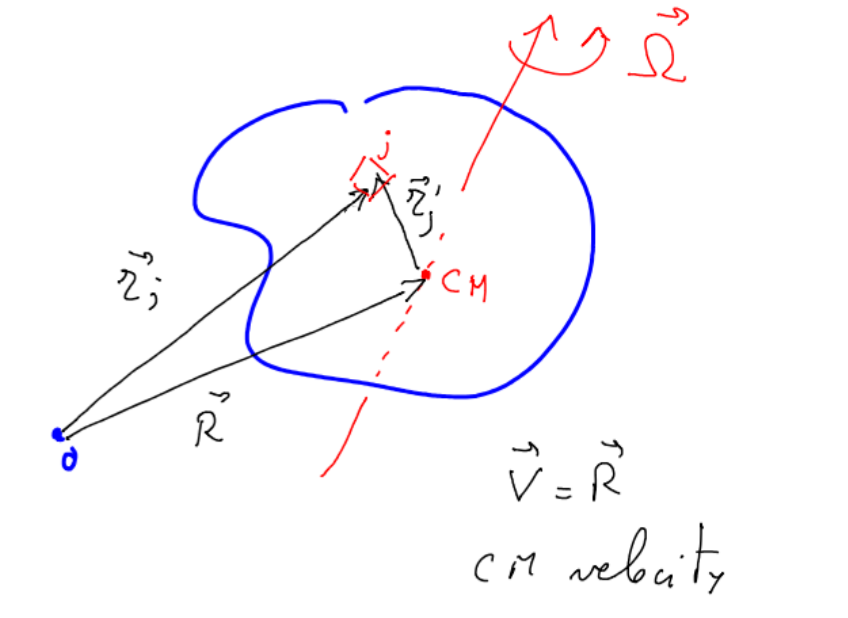
\includegraphics[width=0.6\textwidth]{Images/image006.png}
    \begin{tikzpicture}[shorten >=1pt,node distance=3cm,auto]
        \tikzstyle{every state}=[fill={rgb:black,1;white,10},font=\bfseries]
        \tikzset{every loop/.style={min distance=5mm,in=110,out=70,looseness=5}}
        \node[state] (q0) {0};
        \node[state, right of=q0] (q1) {1};
        \node[state, right of=q1] (q2) {2};
        \node[state, right of=q2] (q3) {3};
        \node[right of=q3] (q4) {$\cdots$};
        \path[->]
        (q0) edge[loop above] node{$p_0$} (q0)
        (q0) edge[bend left] node{$1-p_0$} (q1)
        (q1) edge[bend left] node{$1-p_1$} (q2)
        (q2) edge[bend left] node{$1-p_2$} (q3)
        (q3) edge[bend left] node{$1-p_3$} (q4)
        (q1) edge[bend left, above] node{$p_1$} (q0)
        (q2) edge[bend left, above] node{$p_2$} (q0)
        (q3) edge[bend left, above] node{$p_3$} (q0);
    \end{tikzpicture}
    \caption{Block diagram for the \textit{success run} Markov Chain \label{fig:success-run2}}
\end{figure}

\begin{thm}\label{lemma:product-sum}
    If $0 < p_i < 1$, $i \in \mathbb{N}$, then:
    \begin{align*}
        u_m = \prod_{i=0}^m (1-p_i)  \xrightarrow[m \to \infty]{}  0 \Leftrightarrow \sum_{i=0}^\infty p_i = \infty
    \end{align*}
\end{thm}

\begin{proof}
    Suppose that:
    \begin{align}\label{eqn:hyp1}
        \sum_{i=0}^\infty p_i = \infty
    \end{align}
    Then:
    \begin{align}\label{eqn:exp-ineq}
        1-p_i < 1 - p_i + \frac{p_i^2}{2!} - \frac{p_i^3}{3!} + \dots = e^{-p_i}  \qquad i \in \mathbb{N} 
    \end{align}
    In fact $y = 1-x$ is the tangent of $y = e^{-x}$ at $x=0$, and because $e^{-x}$ is \textit{convex}, it is always higher than its tangents.
    
    Since (\ref{eqn:exp-ineq}) holds for any $i$, it holds also for the product:
    \begin{align*}
        \prod_{i=0}^m (1 - p_i) < \exp\left(-\sum_{i=0}^{m} p_i \right)  \xrightarrow[m \to \infty]{(\ref{eqn:hyp1})}  0
    \end{align*}
    And so we have proved:
    \begin{align*}
        \sum_{i=0}^\infty p_i = \infty \Rightarrow \prod_{i=0}^\infty (1-p_i) = 0
    \end{align*}
    To prove the converse, we assume:
    \begin{align}
        \label{eqn:hyp2}
        \lim_{m \to \infty}\prod_{i=0}^m (1-p_i) = 0
    \end{align}
    Then we make use of the following inequality:
    \begin{align}\label{eqn:ineq3}
        \prod_{i=j}^m (1 - p_i) > (1-p_j - p_{j+1} - \cdots - p_m) = 1 - \sum_{i=j}^m p_i \qquad m \geq j+1
    \end{align}
    which can be proved by induction. It holds for $m = j+1$:
    \begin{align*}
        (1 - p_i)(1-p_{j+1}) = 1 - p_j - p_{j+1} + p_j p_{j+1} > 1 - p_j - p_{j+1}
    \end{align*}
    because all the $p_k$ are non-zero, and so $p_j p_{j+1} > 0$.

    So, assuming it holds for $m$, we can prove that it holds for $m+1$:
    \begin{align*}
        \prod_{i=j}^{m+1} (1- p_i) &= (1-p_{m+1}) \prod_{i=j}^m (1-p_i) \underset{(\ref{eqn:ineq3})}{>} (1-p_{m+1}) \left(1- \sum_{i=j}^m p_i\right) =\\
        &= 1 - \sum_{i=j}^m p_i - p_{m+1} + \underbrace{p_{m+1} \sum_{i=j}^m p_i}_{> 0}  > 1 - \sum_{i=j}^{m+1} p_i
    \end{align*}
    and so it is true for every $m$.

    Then we proceed by contradiction. Suppose that the sum (\ref{eqn:hyp1}) actually converges:
    \begin{align}\label{eqn:con-thesis}
        \sum_{i=0}^\infty p_i < \infty
    \end{align}
    This means that the tail sum must vanish:
    \begin{align*}
        \lim_{j \to \infty} \sum_{i=j}^\infty p_i = 0
    \end{align*}
    So it must become arbitrarily small, and in particular it must be \textit{definitely} between $0$ and $1$:
    \begin{align}\label{eqn:01}
        \exists j_0 > 1 \text{ s.t. } 0 < \sum_{i=j}^\infty p_i < 1 \quad \forall j > j_0
    \end{align} 
    But in that case, applying (\ref{eqn:ineq3}) leads to:
    \begin{align}\label{eqn:conc1}
        \lim_{m \to \infty} \prod_{i=j}^m (1-p_i) > \lim_{m \to \infty} \Bigg(1- \underbrace{\sum_{i=j}^m p_i}_{\mathclap{<1}} \Bigg) > 0
    \end{align}
    Now note that the lhs of (\ref{eqn:conc1}) differs from (\ref{eqn:hyp2}) by only a finite number of non-zero factors (because the $p_i \neq 1$). So:
    \begin{align*}
        \lim_{m \to \infty} \prod_{i=j}^m (1-p_i) > 0 \Rightarrow \lim_{m \to \infty} \prod_{i=\textcolor{Red}{0}}^\infty(1-p_i) > 0
    \end{align*}
    But this contradicts our hypothesis (\ref{eqn:hyp2}), meaning that (\ref{eqn:con-thesis}) cannot be true, and so:
    \begin{align*}
        \prod_{i=0}^\infty (1-p_i) = 0 \Rightarrow \sum_{i=0}^\infty p_i = \infty
    \end{align*}
    which concludes the proof.

\end{proof}
\end{document}
